\documentclass[tikz,border=7pt]{standalone}

\usepackage{amsmath}
\usepackage{bm}
\usetikzlibrary{arrows.meta,calc}

% Colours chosen to match the general maximal-coordinate multibody figure.
\definecolor{frameblue}{RGB}{48,52,255}
\definecolor{rhovector}{RGB}{238,132,24}
\definecolor{torquered}{RGB}{205,35,45}
\definecolor{linkfill}{RGB}{249,249,249}

\tikzset{
  linkbody/.style={
    draw=black,
    fill=linkfill,
    line width=0.85pt,
    rounded corners=3.0mm
  },
  frameaxis/.style={
    draw=frameblue,
    line width=1.15pt,
    line cap=round,
    -{Stealth[length=2.35mm,width=1.85mm]}
  },
  rhoarrow/.style={
    draw=rhovector,
    line width=1.20pt,
    line cap=round,
    -{Stealth[length=2.35mm,width=1.85mm]},
    shorten >=2.2pt
  },
  torquering/.style={
    draw=torquered,
    line width=1.25pt,
    line cap=round
  }
}

\begin{document}
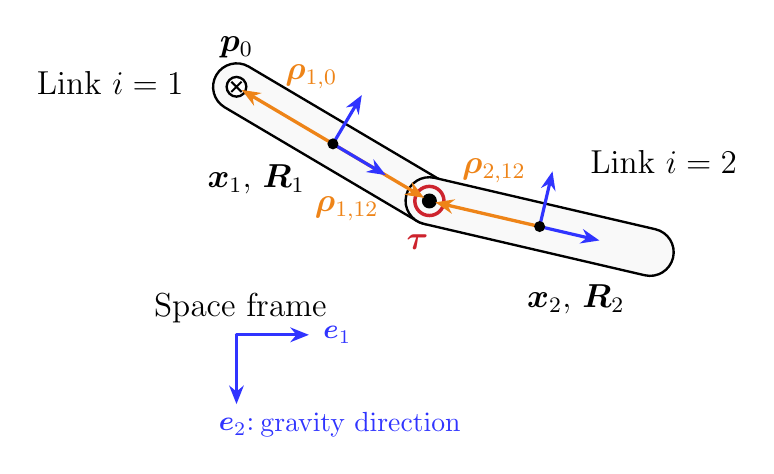
\begin{tikzpicture}[x=1cm,y=1cm]

  % Joint positions and centers of mass in the global frame.
  \coordinate (P0)  at (-2.45, 1.45);
  \coordinate (P12) at ( 0.00, 0.00);
  \coordinate (C1)  at (-1.225,0.725);
  \coordinate (C2)  at ( 1.40,-0.325);
  \coordinate (G)   at (-2.45,-1.70);

  % Link i=1 is drawn first.
  \begin{scope}[shift={(C1)},rotate=-30.6]
    \path[linkbody] (-1.72,-0.30) rectangle (1.72,0.30);
  \end{scope}

  % Link i=2 is drawn afterwards and therefore appears above link i=1.
  \begin{scope}[shift={(C2)},rotate=-13.1]
    \path[linkbody] (-1.74,-0.30) rectangle (1.74,0.30);
  \end{scope}

  % Fixed base joint p_0.
  \draw[black,line width=0.85pt,fill=white] (P0) circle[radius=0.125];
  \draw[black,line width=0.75pt]
    ($(P0)+(-0.065,-0.065)$) -- ($(P0)+(0.065,0.065)$)
    ($(P0)+(-0.065, 0.065)$) -- ($(P0)+(0.065,-0.065)$);

  % Elbow joint.
  \fill[black] (P12) circle[radius=0.095];

  % Elbow torque is indicated by a red ring around the actuated joint.
  \draw[torquering] (P12) circle[radius=0.185];
  \node[text=torquered,font=\large] at (-0.15,-0.52) {$\bm{\tau}$};

  % Body-fixed offset vectors are drawn below the body-fixed frames.
  \draw[rhoarrow] (C1) -- (P0);
  \draw[rhoarrow] (C1) -- (P12);
  \draw[rhoarrow] (C2) -- (P12);

  \node[text=rhovector,font=\large] at (-1.50,1.58)
    {$\bm{\rho}_{1,0}$};
  \node[text=rhovector,font=\large] at (-1.05,-0.10)
    {$\bm{\rho}_{1,12}$};
  \node[text=rhovector,font=\large] at ( 0.82, 0.38)
    {$\bm{\rho}_{2,12}$};

  % Body-fixed planar coordinate frame at the center of mass of link i=1.
  \begin{scope}[shift={(C1)},rotate=-30.6]
    \draw[frameaxis] (0,0) -- (0.78,0);
    \draw[frameaxis] (0,0) -- (0,0.72);
  \end{scope}

  % Body-fixed planar coordinate frame at the center of mass of link i=2.
  \begin{scope}[shift={(C2)},rotate=-13.1]
    \draw[frameaxis] (0,0) -- (0.78,0);
    \draw[frameaxis] (0,0) -- (0,0.72);
  \end{scope}

  \fill[black] (C1) circle[radius=0.07];
  \fill[black] (C2) circle[radius=0.07];

  % Body, state, and base-position labels remain black.
  \node[font=\large,anchor=east] at (-3.00,1.50) {Link $i=1$};
  \node[font=\large,anchor=west] at ( 1.92,0.50) {Link $i=2$};
  \node[font=\large] at (-2.20,0.28) {$\bm{x}_{1},\,\bm{R}_{1}$};
  \node[font=\large] at ( 1.86,-1.25) {$\bm{x}_{2},\,\bm{R}_{2}$};
  \node[font=\large,anchor=south] at ($(P0)+(0,0.24)$) {$\bm{p}_{0}$};

  % Space-fixed planar coordinate frame.
  \draw[frameaxis] (G) -- ++(0.92,0);
  \draw[frameaxis] (G) -- ++(0,-0.88);
  \node[text=frameblue,font=\normalsize,anchor=west]
    at ($(G)+(0.98,0)$) {$\bm{e}_{1}$};
  \node[text=frameblue,font=\normalsize,anchor=north]
    at ($(G)+(0,-0.94)$) {$\bm{e}_{2}$:};
  \node[text=frameblue,font=\normalsize,anchor=west]
    at ($(G)+(0.18,-1.14)$) {gravity direction};
  \node[font=\large,anchor=north] at ($(G)+(0.05,0.65)$) {Space frame};

\end{tikzpicture}
\end{document}
